\documentclass{rapport}
\usepackage{pythontex}
\usepackage{csquotes}
\addbibresource{library.bib}
\title{Rapport laboratoire de matériaux : nickelage} %Titre du fichier

\begin{document}

%----------- Informations du rapport ---------

\unif{HEIG}
\titre{Conception d'un système automatisé permettant le cassage de microcapsules en verre et la libération contrôlée de réactifs chimiques} %Titre du fichier .pdf
\cours{Travail de bachelor} %Nom du cours
\sujet{Laboratoire Swiss cat +} %Nom du sujet


\enseignant{Giuseppe \textsc{Costanzo}}%Nom de l'enseignant

\eleves{Arnaud \textsc{Arpino} } %Nom des élèves

\entreprise{EPFL - Swiss Cat + \\
Keyan VILLAT\\
Henryk ZOLNOWSKI
}

\nom{Arnaud ARPINO}

%----------- Initialisation -------------------
        
\fairemarges %Afficher les marges
\fairepagedegarde %Créer la page de garde

\pagenumbering{roman} 
\clearpage
\null
\thispagestyle{empty}
\clearpage

\vspace*{4cm}
\section*{\Huge Préambule}
\addcontentsline{toc}{section}{Préambule} % Ajout à la table des matières

\vspace{1cm}
Ce travail de Bachelor (ci-après TB) est réalisé en fin de cursus d'études, en vue de
l'obtention du titre de Bachelor of Science HES-SO en Ingénierie.
En tant que travail académique, son contenu, sans préjuger de sa valeur, n'engage
ni la responsabilité de l'auteur, ni celles du jury du travail de Bachelor et de l'École.
Toute utilisation, même partielle, de ce TB doit être faite dans le respect du droit
d'auteur.

\vspace{2cm}

\hspace*{10cm}
\begin{minipage}{0.3\textwidth}
    HEIG-VD\\
    Le Chef du Département
\end{minipage}

\vspace{5cm}
Yverdon-les-bains, le \today

\clearpage
\null
\thispagestyle{empty}
\clearpage
\newpage

\vspace*{4cm}
\section*{\Huge Authentification}
\addcontentsline{toc}{section}{Authentification}

\vspace{2cm}
Je soussigné, Arnaud Arpino, atteste par la présente avoir réalisé seul ce travail et
n'avoir utilisé aucune autre source que celles expressément mentionnées.

\vspace{2cm}

\hspace*{10cm}
\begin{minipage}{0.3\textwidth}
    Arnaud ARPINO\\
    
\includegraphics[height=3cm]{Images/Signatures/signature Arnaud.png}
\end{minipage}

\vspace{5cm}
Yverdon-les-bains, le \today

\newpage

\clearpage
\null
\thispagestyle{empty}
\clearpage
\newpage

\vspace*{1cm}
\section*{\Huge Complémentaire concernant \\
l'utilisation d'outils\\
d'intelligence artificielle}
\addcontentsline{toc}{section}{Complémentaire concernant l'utilisation d'outils d'intelligence artificielle}

\vspace{2cm}

L'utilisation limitée d'outils dits d'intelligence artificielle ou plus particulièrement de
LLM (Large Language Models) a été validée avant le début de ce travail de bachelor
pour les utilisations spécifiques suivantes :

\vspace{1cm}
Utilisation de ChatGPT de l'entreprise OpenAI versions GPT-3, GPT-4 et ChatGPT-4-turbo pour
obtenir rapidement des informations servant de double vérifications, de correction
orthographique, de reformulation lors de la rédaction, d'aide pour le language LATEX, d'aide pour les langages de programmation python et 
autres langages utiles à la programmation du bras robotisé robot. 


\vspace{1cm}
Je soussigné, M. Arnaud Arpino, atteste par la présente avoir nullement utilisé de
logiciels de génération de texte automatique pour la rédaction de ce document sans réflexion personnel
au préalable et que toutes les resources spécifiques utilisées se trouvent dans la bibliographie ou en
annexe de ce rapport.

\vspace{2cm}

\hspace*{10cm}
\begin{minipage}{0.3\textwidth}
    Arnaud ARPINO\\
    
\includegraphics[height=3cm]{Images/Signatures/signature Arnaud.png}
\end{minipage}

\vspace{1cm}
Yverdon-les-bains, le \today



\newpage

\clearpage
\null
\thispagestyle{empty}
\clearpage
\newpage

\section*{\Huge Résumé}
\addcontentsline{toc}{section}{Résumé}

\clearpage
\null
\thispagestyle{empty}
\clearpage
\newpage 

\clearpage
\pagestyle{plain} 

\thispagestyle{roman}
\tabledematieres %Créer la table de matières
\newpage

\thispagestyle{roman}
\listoftables
\newpage

\thispagestyle{roman}
\listoffigures

\clearpage
\pagenumbering{arabic} 
\pagestyle{fancy}
\setcounter{page}{1}

%------------ Corps du rapport ----------------

\section{Introduction}

\subsection{Contexte}
Dans le cadre de formation de microtechnicien, l'étudiant doit réaliser un Travail de Bachelor pour valider ses compétences. L'avancement de ce travail peut se déroulé à l'HEIG salle C26, au laboratoire Swiss Cat + de l'EPFL ou à distance, selon les règles établies par les enseignants et responsables des locaux. Le projet doit être réalisé sur une durée de 420 heures, réparties entre mi février et la fin du mois de juillet.

\subsection{Description du projet}

\subsection{Organisation}


\newpage
\section{Cahier des charges}

\subsection{Définitions}

\begin{itemize}[label=\textbullet]
    \item \textbf{Micro-capsules}: petit cylindres en verre fermés des deux côtés (borosilicate). \\ 
    Diamètre extérieur = 2,8 ± 0,05 mm; \\
    Diamètre intérieur = 2,5 ± 0,05 mm; \\
    Longueur = 10 mm

    \item \textbf{Réacteurs}: Flacons à sertir en verre dimension: 11 mm, 12 x 32, 2 ml 
    
    \item \textbf{Bloc de réaction}: Plaques « Para-Dox » avec 48 positions, Gen II, pour flacons 12 x 32
\end{itemize}

\subsection{Analyse du besoin}

\begin{figure}[H]
    \centering
    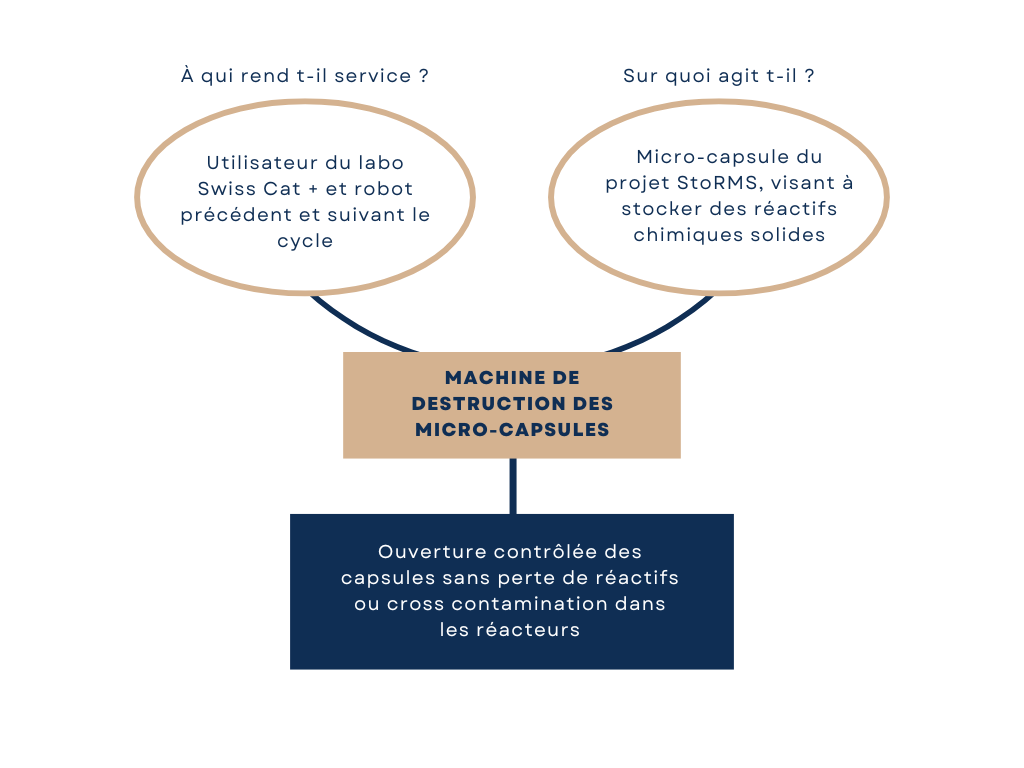
\includegraphics[width=15cm]{Images/Illustrations/CDH/Bete a corne.png}
    \label{fig:beteacorne}
    \caption{Diagramme bête à corne}
\end{figure}

\begin{table}[H]
    \centering
    \begin{tabular}{
    >{\columncolor[HTML]{FFFFFF}}l |
    >{\columncolor[HTML]{FFFFFF}}l }
    {\color[HTML]{000000} \textbf{\#}} & {\color[HTML]{000000} \textbf{Besoin}}           \\ \hline
    {\color[HTML]{000000} \textbf{1}} & {\color[HTML]{000000} Ouvrir des micro-capsules} \\ \hline
    {\color[HTML]{000000} \textbf{2}} & {\color[HTML]{000000} } \\ \hline
    {\color[HTML]{000000} \textbf{}}  & {\color[HTML]{000000} } \\ \hline
    \end{tabular}
    \caption{Liste des besoins du système}
    \label{tab:besoin}
    \end{table}

\subsection{Fonctions et exigences du système}
\subsubsection{Fonctions de services}

Les fonctions de services correspondes aux exigences principales du produits (réflexions basé sur cahier des charges du projet multi 2024 \cite{projmulti2024}).


\begin{table}[H]
    \centering
    \begin{tabular}{
    >{\columncolor[HTML]{FFFFFF}}l 
    >{\columncolor[HTML]{FFFFFF}}l |
    >{\columncolor[HTML]{FFFFFF}}l 
    >{\columncolor[HTML]{FFFFFF}}l }
    \multicolumn{2}{l|}{\cellcolor[HTML]{FFFFFF}{\color[HTML]{000000} \textbf{Fonctions de service}}} &
      \multicolumn{2}{l}{\cellcolor[HTML]{FFFFFF}{\color[HTML]{000000} \textbf{Exigences}}} \\ \hline
    \multicolumn{1}{l|}{\cellcolor[HTML]{FFFFFF}{\color[HTML]{000000} \textbf{FS 1}}} &
      {\color[HTML]{000000} \begin{tabular}[c]{@{}l@{}}Doit être en mesure \\ de détruire une micro-capsule\end{tabular}} &
      \multicolumn{1}{l|}{\cellcolor[HTML]{FFFFFF}{\color[HTML]{000000} \textbf{E 1}}} &
      {\color[HTML]{000000} \begin{tabular}[c]{@{}l@{}}Libération totale du réactif \\ (débris de verres inclus)\end{tabular}} \\ \hline
    \multicolumn{1}{l|}{\cellcolor[HTML]{FFFFFF}{\color[HTML]{000000} \textbf{FS 2}}} &
      {\color[HTML]{000000} \begin{tabular}[c]{@{}l@{}}Doit être en capable \\ de répéter la tâche\end{tabular}} &
      \multicolumn{1}{l|}{\cellcolor[HTML]{FFFFFF}{\color[HTML]{000000} \textbf{E 2}}} &
      \cellcolor[HTML]{FFFFFF}{\color[HTML]{000000} \begin{tabular}[c]{@{}l@{}}Répétabilité de la tâche \\ 48 fois par plaque\end{tabular}} \\ \hline
    \multicolumn{1}{l|}{\cellcolor[HTML]{FFFFFF}{\color[HTML]{000000} \textbf{FS 3}}} &
      {\color[HTML]{000000} } &
      \multicolumn{1}{l|}{\cellcolor[HTML]{FFFFFF}{\color[HTML]{000000} \textbf{E 3}}} &
      {\color[HTML]{000000} }
    \end{tabular}
    \caption{Fonctions de service}
    \label{tab:fctservice}
    \end{table}

\subsubsection{Fonctions techniques}

\begin{table}[H]
  \centering
  \begin{tabular}{cl|cl}
  \multicolumn{2}{l|}{\textbf{Fonctions techniques}}                   & \multicolumn{2}{l}{\textbf{Exigences}}                                         \\ \hline
  \multicolumn{1}{c|}{\textbf{FT 1}} &
    \begin{tabular}[c]{@{}l@{}}Doit fonctionner dans \\ un environnement contrôlé.\end{tabular} &
    \multicolumn{1}{c|}{\textbf{E 5}} &
    \begin{tabular}[c]{@{}l@{}}Glove box rempli uniquement \\ d'azote à température ambiante.\end{tabular} \\ \hline
  \multicolumn{1}{c|}{\textbf{FT 2}} & Doit être simple d'utilisation. & \multicolumn{1}{c|}{\textbf{E 6}} & Mise en place par un laborantin de chimie. \\ \hline
  \multicolumn{1}{c|}{\textbf{FT 3}} &
    \begin{tabular}[c]{@{}l@{}}Doit assurer la sécurité de \\ l'utilisateur et de des équipements \\ lors du fonctionnement.\end{tabular} &
    \multicolumn{1}{c|}{\textbf{E 7}} &
    \begin{tabular}[c]{@{}l@{}}Protection contre projection, \\ capteur ou système de sécurité \\ en cas de défaillance ou conditions anormale.\end{tabular} \\ \hline
  \multicolumn{1}{c|}{\textbf{FT 4}} &                                 & \multicolumn{1}{c|}{\textbf{E 8}} &                                           
  \end{tabular}
  \caption{Fonctions techniques}
  \label{tab:fctstechnique}
  \end{table}



\subsubsection{Fonctions de contraintes}

\begin{table}[H]
  \centering
  \begin{tabular}{cl|cl}
  \multicolumn{2}{l|}{\textbf{Fonctions de contrainte}}                   & \multicolumn{2}{l}{\textbf{Exigences}}                       \\ \hline
  \multicolumn{1}{c|}{\textbf{FC 1}} & Doit éviter la cross contamination & \multicolumn{1}{c|}{\textbf{E 9}}  & Système anti-projection \\ \hline
  \multicolumn{1}{c|}{\textbf{FC 2}} &                                    & \multicolumn{1}{c|}{\textbf{E 10}} &                        
  \end{tabular}
  \caption{Fonctions de contrainte}
  \label{tab:fctscontr}
  \end{table}







\section{Catalogue des solutions}

\subsection{Liste des solutions envisagées}
\subsubsection{Canon à azote}


\subsubsection{Implosion de la capsule}



\subsubsection{Actionneur mécanique}



\input{Chapitres/98-Signatures}
%%------------- Commandes utiles ----------------

\section{Quelques commandes}

Voici quelques commandes utiles :

%------ Pour insérer et citer une image centralisée -----

\insererfigure{logos/Import.jpg}{3cm}{Légende de la figure}{Label de la figure}
% Le premier argument est le chemin pour la photo
% Le deuxième est la hauteur de la photo
% Le troisième la légende
% Le quatrième le label
Ici, je cite l'image \ref{fig: Label de la figure}


%------- Pour insérer et citer une équation --------------

\begin{equation} \label{eq: exemple}
\rho + \Delta = 42
\end{equation}

L'équation \ref{eq: exemple} est cité ici. 

% ------- Pour écrire des variables ----------------------

Pour écrire des variables dans le texte, il suffit de mettre le symbole \$ entre le texte souhaité comme : constante $\rho$.

Pour utiliser pythontex : (pour les chapitres un fichier tex séparé pour python a été préparé)
\begin{pycode}
x = 3
\end{pycode}
       
$x = \py{x}$

si x = ?? effectuer :
pythontex main.tex


Pour créer une bibliographie avec des citations :

Ceci est du texte avec une citation complète comme note de bas de page.\footfullcite{smith2023}
Ceci est une référence d'un site \footfullcite{Biscactus}
Ceci est une référence d'un site \footfullcite{LaTeX}


\newpage
\printbibliography % To generate the bibliography
\appendix
%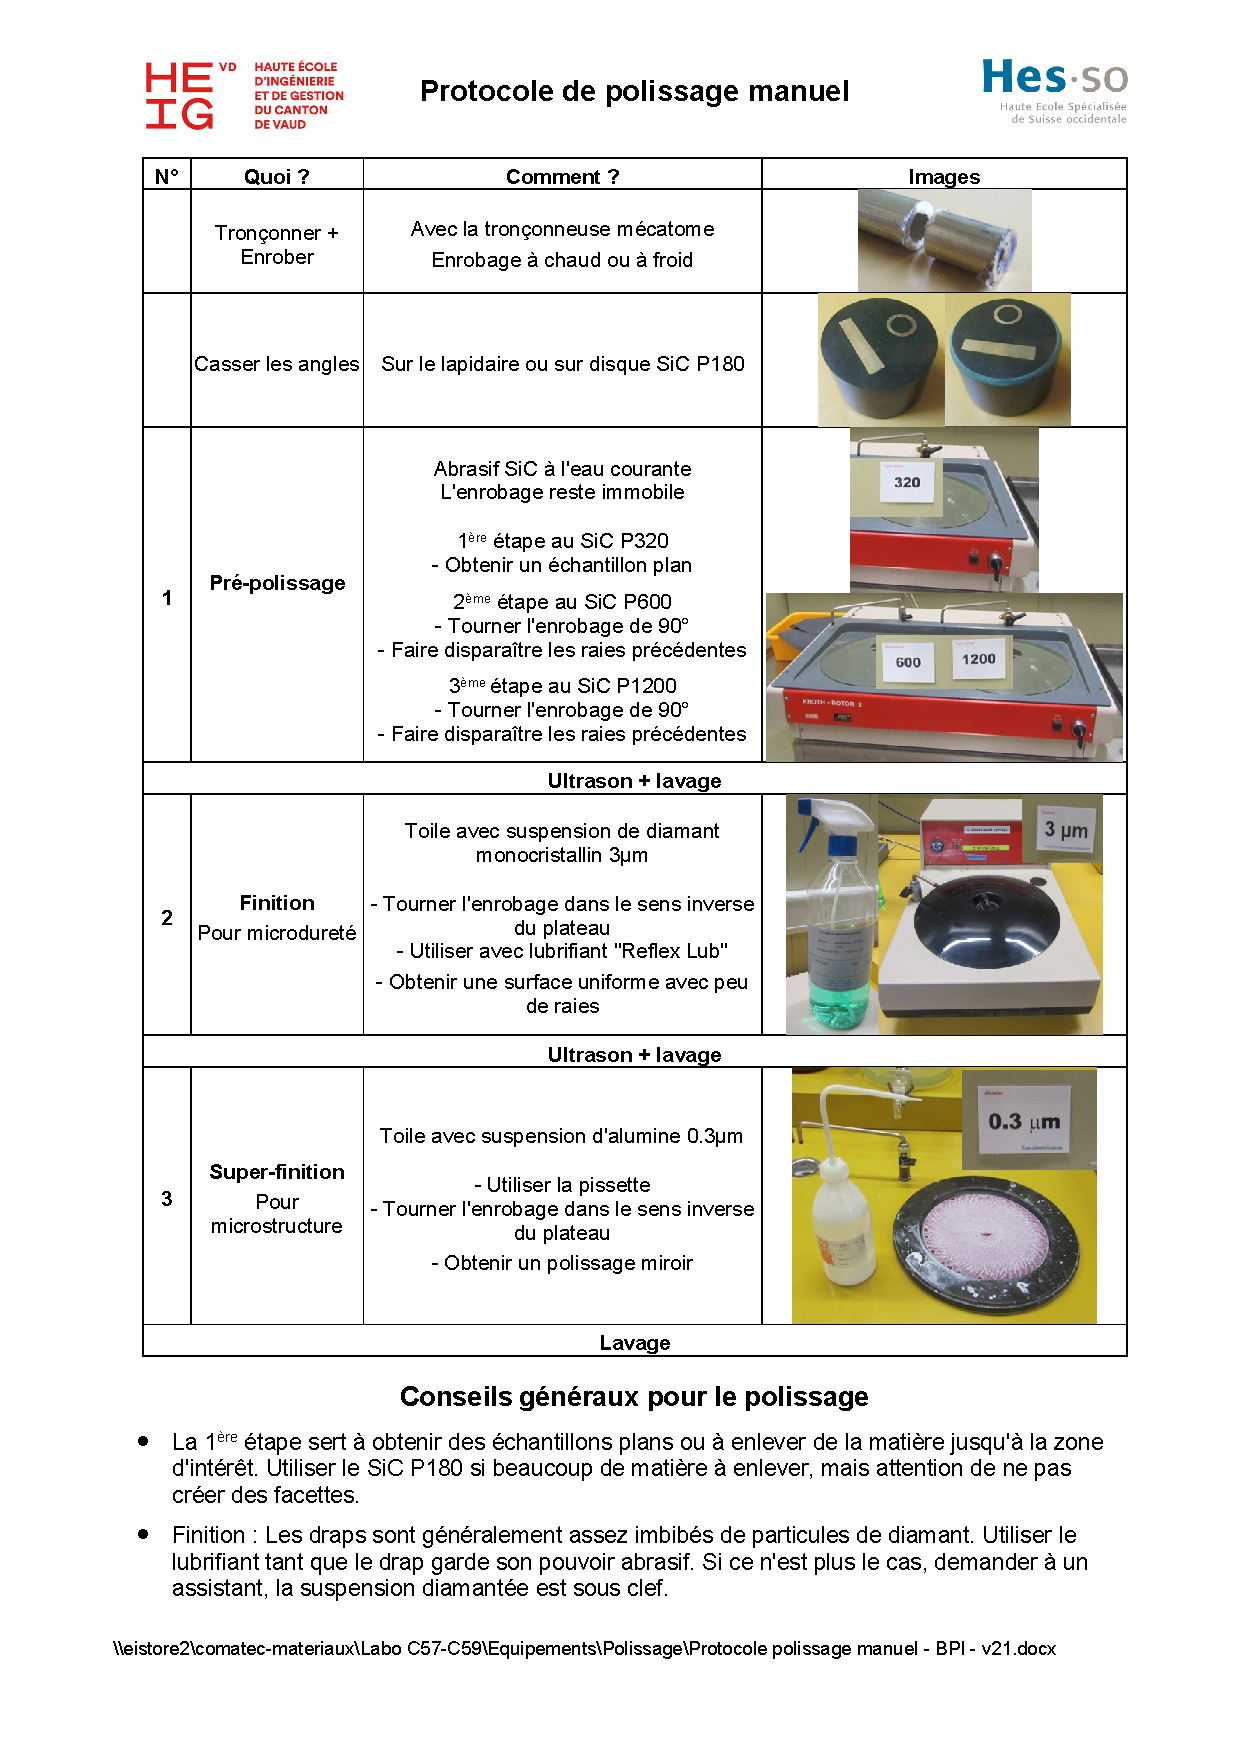
\includepdf[pages=1,pagecommand={\thispagestyle{empty}\vspace*{-4.8cm}\section{Protocole de polissage}\label{pdf: polissage}}]{pdfs/TP03 Protocole polissage manuel.pdf}
%\includepdf[pages=2]{pdfs/TP03 Protocole polissage manuel.pdf}


\end{document}